\begin{figure}
\centering
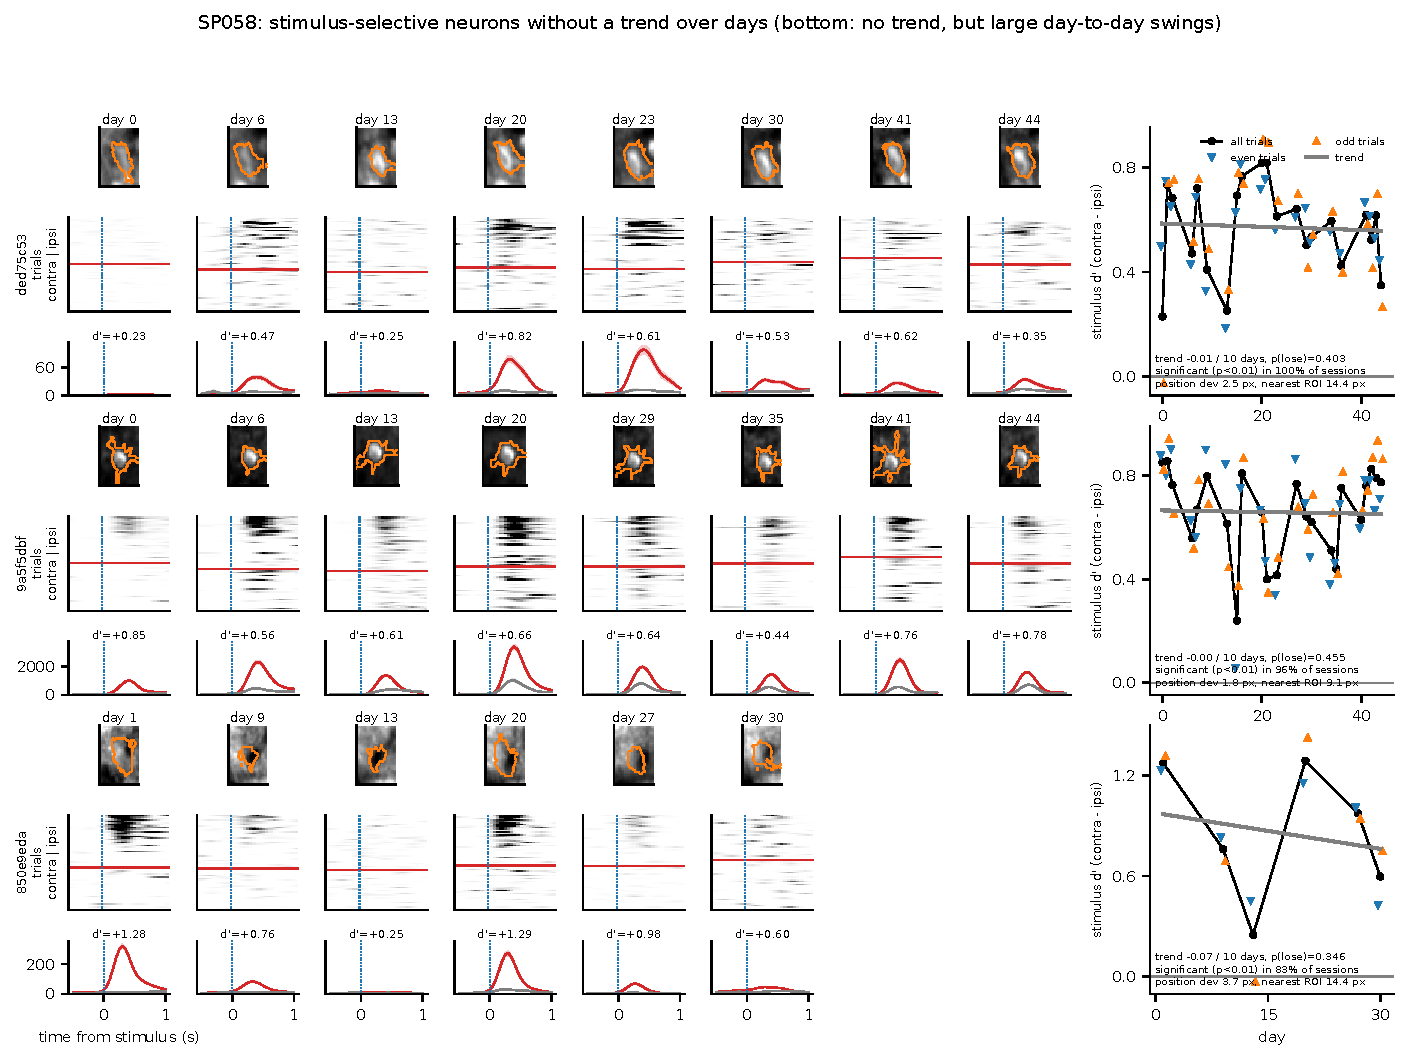
\includegraphics[width=\textwidth]{examples_stable.pdf}\\[2mm]
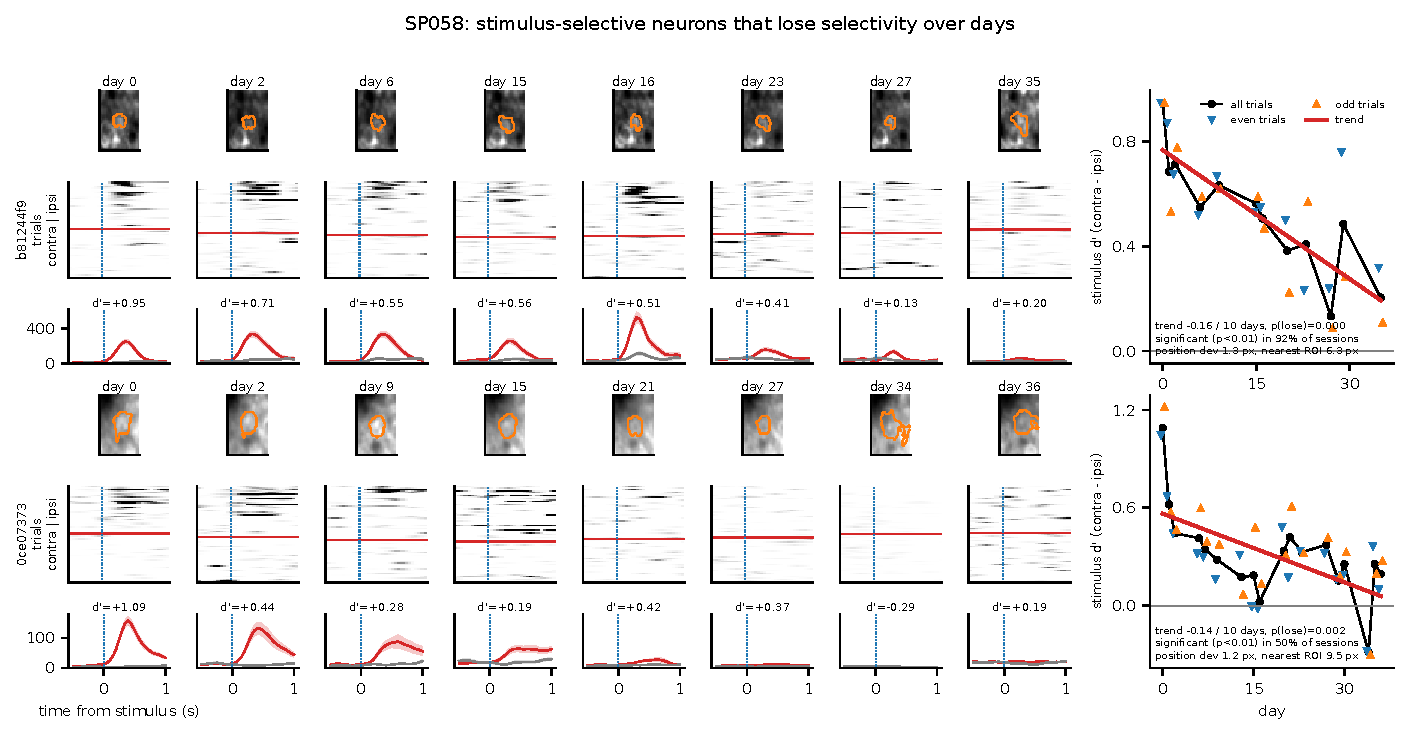
\includegraphics[width=\textwidth]{examples_losing.pdf}
\caption{\textbf{Example tracked neurons (SP058) that keep or lose their stimulus selectivity.} Per neuron, columns are up to 8 of its tracked sessions. Top row: mean image around the ROI with the ROI outline. Middle: deconvolved activity around stimulus onset, trials with a contralateral stimulus above the red line, ipsilateral below, sorted by contrast. Bottom: mean $\pm$ s.e.m.\ (red: contra, grey: ipsi) and the session's d$'$. Right: d$'$ (contra $-$ ipsi, 0--0.3~s) in every tracked session, from all, even and odd trials, with the linear trend and its session-shuffle permutation $p$. Top figure: no trend (bottom neuron: no trend but large day-to-day changes that even and odd trials agree on). Bottom figure: significant loss of selectivity.}
\label{fig:examples}
\end{figure}
